\chapter{Secure Differentially Private Mechanisms On Finite Computer}
\label{cha:secureDPMechanisms}

Generally, the security analysis of differentially private mechanisms is based on two implicit assumptions: (i) Computations are performed on real numbers and requires machines to have infinite precision, (ii) The noise is sampled from a probability distribution very close to the theoretically correct probability distribution. However, the practical implementataion of differentially private mechanisms are based on floating-point or fixed-point arithmetic that only provides finite order of accuracy. Mironov \cite{mironov2012significance} showed that the porous distribution of the Laplace random noise sampled with textbook algorithm under floating-point implemetation can lead to violation of differential privacy. In this chapter, we describe four types of existing differentially private mechanisms~\cite{mironov2012significance,googleDP2019,ghosh2012universally,canonne2020discrete} and modify corresponding algorithms for sampling secure random noise on finite computer. We construct MPC protocols for these differentially private mechanisms and sampling algorithms in~\autoref{cha:MPCProtocolsforDifferentiallyPrivateMechanisms}.



% Recall that differentially private mechanisms (cf.~\autoref{subsec:DPMechanisms}) guarantee differential privacy by adding appropriately chosen random noise to a query function $f\left(D\right)  $, which can be expressed as:

% \[M\left(D\right)=f\left(D\right)+Y,\]

% where $D$ is the database, $Y $ is the noise term.




However, we only have machines with finite-precision for the practical implementations of differentially private mechanisms. We typically use fixed-point or floating-point arithmetic to approximate the operations of real numbers. Mironov~\cite{mironov2012significance} shows that the porous distribution of the Laplace noise implemented with the textbook noise sampling methods under floating-point arithmetic can lead to severe differential privacy breaching and proposes the snapping mechanism to avoid such security issues by rounding and smoothing the output of the Laplace Mechanism (cf.~\autoref{def:laplaceMechanism}). \CHANGED{Google Differential Privacy Team~\cite{googleDP2019} introduces an alternative secure approach that scales integer noise from certain distribution under floating-point arithmetic to approximate continuous noise in desired distribution and yields better accuracy than the snapping mechanism}. \CHANGED{Canonne et al.~\cite{canonne2020discrete} provide algorithms to sample discrete Laplace and Gaussian noise on finite computer for the query function $f\left(D\right) \in \mathbb{Z} $}.


\section{Snapping Mechanism}
\label{sec:snappingMechanism}
Recall that Laplace mechanisms (cf.~\autoref{subsec:DPMechanisms}) guarantee $\varepsilon$ differential privacy by adding Laplace random variable to the query function $f\left(D\right)  $:
\begin{equation}
    \begin{split}
        M\left(D, \lambda\right)=f\left(D\right)+Y,
    \end{split}
\end{equation}

where $D$ is the database and $Y \sim Lap\left(\lambda\right) $.

As discussed in \autoref{algo:textLaplaceSamplingAlgorithm}, we can generated a Laplace random variable $Y$ by transforming the random chosen sign $S\in \left\{-1,1\right\} $ and a uniform random variable $U \in \left(0,1\right] $ (or $U \in \left(0,1\right) $ if we ignore the \textit(small) probability of genereating the exact $1$) as follows:
\begin{equation}
    \begin{split}
        Y \gets S \cdot \lambda \ln\left(U\right)
    \end{split}
\end{equation}


Mironov~\cite{mironov2012significance} showed that the Laplace random variable $Y$ generated in this method under floating-point arithmetic can lead to severe differential privacy breaching and proposed the snapping mechanism to avoid such security issues by rounding and smoothing the output $f\left(D\right)+Y$.

% In this section, we describe the snapping mechanism that is immune to the attack
% \CHANGED{Laplace random variable $Y \sim Lap\left(\lambda\right) $ (cf.~\autoref{def:LaplaceDistribution}) can be generated with the inverse transform sampling method (cf.~\autoref{theorem:inversionSamplingMethod}):}
% \begin{equation}
%     \begin{split}
%         % Y&=\left(2Z-1\right)\cdot b \ln\left(1-U\right)\\
%         Y&=S\cdot \lambda \ln\left(U\right),
%     \end{split}
% \end{equation}
% where $S\in \left\{-1,+1\right\} $ is the sign, $\lambda$ controls the magnitude of $Y$, and $U$ is a uniform random variable in interval $(0,1]$.

% Mironov~\cite{mironov2012significance} demonstrates an attack on the floating-point implementation of the Laplace mechanism (cf.~\autoref{def:laplaceMechanism}) based on the above noise generation method and proposes the snapping mechanism $M_S$ to guarantee differential privacy with rounding and clamping operations, that is defined as:

The snapping mechanism is defined as follows:
\begin{equation}
    \begin{split}
        M_{S}\left(f\left(D\right),\lambda,B\right) =\text{clamp}_{B}\left(\left\lfloor\text {clamp }_{B}\left(f\left(D\right) \right) \oplus S\otimes \lambda\otimes \text{LN}\left(U^{*}\right) \right\rceil_{\Lambda}\right).
    \end{split}
\end{equation}

% \TODO{explain exact rounding}

Let $\mathbb{D}$ denote the set of floating-point numbers, and $\mathbb{D} \cap \left(a,b\right) $ denote all the floating-point numbers in the interval $\left(a,b\right)$.
$f\left(D\right) \in \mathbb{D} $ is the query function of database $D$, and $S\otimes \lambda\otimes \text{LN}\left(U^{*}\right)$ is the noise term.
$S$ is the sign of the noise that is uniformly distributed over $\left\{-1,1\right\} $. $U^{*}$ is a \textit{uniform} distribution over $\mathbb{D} \cap \left(0,1\right) $, and generates floating-point numbers with probability proportional to its \textit{unit in the last palce} (ulp), i.e., spacing between two consecutive floating-point numbers. \CHANGED{$\text{LN}(x )$ is the natural logarithm under floating-point implementation with exact rounding, i.e., $\text{LN}(x )$ rounds input $x$ to the closest floating-point number with probability $p=1$.}
$\oplus$ and $\otimes$ are the floating-point implementations of addition and multiplication.

Function $\text{clamp}_{B}\left(x\right) $ limits the output to the interval $\left[-B, B\right] $ by outputting $B$ if $x > B$, $-B$ if $x < -B$, and $x$ otherwise.   $\Lambda$ is the smallest power of two greater than or equal to $\lambda$, and we have $\Lambda=2^{n}$ such that $2^{n-1} < \lambda \leq2^{n}$ for $n \in \mathbb{Z} $. Function $\lfloor x\rceil_{\Lambda}$ rounds input $x$ exactly to the nearest multiple of $\Lambda$ by manipulating the binary floating-point representation of $x$.

Note that the snapping mechanism assumes that the \textit{sensitivity} $\Delta_1 ^{f} $ (cf.~\autoref{def:sensitivity}) of query function $f$ is $1$, which can be extended to an arbitrary query function $f^{\prime}$ with \textit{sensitivity} $\Delta _1^{\left(f^{\prime}\right) }\neq 1$ by scaling the output of $f^{\prime}\left(D\right) $ with $f\left(D\right) =\frac{f^{\prime}\left(D\right) }{\Delta_1 ^{\left(f^{\prime}\right) }}$.

\begin{theorem}[{~\cite{mironov2012significance}}]
    The snapping mechanism $M_{S}\left(f\left(D\right),\lambda,B\right)$ satisfies $\left(\frac{1}{\lambda}+\frac{2^{-49}B}{\lambda}\right) $-DP for query function $f$ with \textit{sensitivity} $\Delta _1^{\left(f\right) } =1$ when $\lambda<B<2^{46}\cdot\lambda$.
\end{theorem}
% \TODO{prove about snapping mechanism DP properties and correctness}

% \subsection{Implementations of Snapping Mechanism}
% \label{subsec:snappingImp}

% We introduce snapping mechanism implementations from~\cite{Covington2019} and adapt them into MPC protocols in~\autoref{sec:snappingMPC}, other implementations of snapping mechanism are known as~\cite{George2017, Ristea2021}.

The snapping mechanism consists of the following steps:
\begin{enumerate}
    \label{enu:snappingSteps}
    \item $\text{clamp}_B\left(\cdot\right) $.
    \item Generation of $U^{*}$ and $S$.
    \item Floating-point arithmetic operations: $\text{LN}\left(\cdot\right) $, $\oplus$, $\otimes $.
          % \item Calculation of $\Lambda$.
    \item $\lfloor x\rceil_{\Lambda}$ that rounds input $x$ to the nearest multiple of $\Lambda $.
\end{enumerate}
We briefly describe how to generate $U^{*}$, the implementation details of the rest steps can be found in the Covington's work~\cite{Covington2019}.


% \subsubsection{Generation of $U^{*}$}
% \label{subsubsec:generationUStar}

\textbf{Generation of $U^{*}$}
$U^{*}$ is a \textit{uniform} distribution over $\mathbb{D} \cap \left(0,1\right) $ and can be represented in IEEE 754 floating-point~\cite{IEEE754_2019} as:
\begin{equation}
    \begin{split}
        U^{*}=\left(1.d_{1}\ldots d_{52}\right)_{2}\times2^{e-1023}.
    \end{split}
\end{equation}

As discussed above, each floating-point $U^{*}$ should be output with a probability proportional to its ulp. We sample a floating-point number from $U^{*}$ using \autoref{algo:RandFloat1}~\cite{walker1974fast,mironov2012significance}, i.e., independently sampling a geometric random variable $x \sim Geo\left(0.5\right) $, and the significant bits $\left(d_{1},\ldots ,d_{52}\right)\in\left\{0,1\right\}^{52} $. Then we set $U^{*}$'s biased exponent $e=1023-\left(x+1\right) $.

\begin{algorithm}[tbh!]
    \centering
    \fbox{
    \pseudocode[space=none, syntaxhighlight=auto, addkeywords={Algorithm, Input, Output, IF,TO,RETURN, FOR, ELSE IF, ELSE, WHILE},linenumbering, skipfirstln, head=\textbf{Algorithm: $Algo^{RandFloat1}$}]{
    \textbf{Input: None} \pcskipln \\
    \textbf{Output: $U^{*}\in \mathbb{D} \cap \left(0,1\right)$} \\
    \text{$\left(d_1,\ldots,d_{52}\right)\sample \left\{0,1\right\}^{52} $}\\
    \text{$x \gets Algo^{Geometric}\left(0.5\right)  $}\\
    \text{$e \gets 1023-\left(x+1\right) $}\\
    \text{RETURN $U^{*}=\left(1.d_1\ldots d_{52}\right)_2 \times 2^{e-1023}$}
    }}
    \caption{Algorithm for sampling random floating-point number $U^{*}\in\left(0,1\right) $.}
    \label{algo:RandFloat1}
\end{algorithm}
\FloatBarrier

As $U^{*}$'s significant bits are sampled randomly from $\left\{0,1\right\}^{52} $, the floating-point numbers with identical biased exponent $e-1023$ are distributed uniformly in $U^{*}$.
Further, $x \sim Geo\left(0.5\right) $ guarantees that the probability of sampling a floating-point number from $U^{*}$ is proportional to its ulp.

Intuitively, \textit{uniformly} sampling a floating-point number can be thought of as first randomly drawing a real number in the interval $\left(0,1\right) $ and rounding it to the nearest floating-point number. However, the floating-point numbers are discrete and not equidistant. For example, there are exactly $2^{52}$ representable reals in interval $[.5, 1)$ and $2^{52}$ reals in interval $[ .25, .5)$. If we only sample the floating-point numbers with equal distance to each other in interval $\left(0,1\right) $, a large part of floating-point numbers would be ignored. As discussed in~\cite{walker1974fast,mironov2012significance}, a better approach is to sample floating-point numbers with probability proportional to its ulp (i.e., spacing to its consecutive neighbor).
With $x\sim Geo\left(0.5\right) $, the total sampling probability for the floating-point numbers in interval $(0,1)$ with exponent $e-1023=-1$ is $Pr\left(x=0 \,|\,0.5\right) =\frac{1}{2}$.
The total sampling probability for the floating-point numbers in interval $(0,0.5)$ with exponent $e-1023=-2$ is $Pr\left(x=1\,|\,0.5\right) =\frac{1}{2^2}$ , etc.
Therefore, we have a total sampling probability for the floating-point numbers in in interval $\left(0,1\right)$ is $\sum_{i = 1}^{\infty}\frac{1}{2^{i}}\approx 1$.


% % \TODO{image about uniform sampling of floating point number}
% \autoref{img::floatingpointdistribution} shows the distribution of floating-point numbers (in form $\left(-1\right)^S\left(1.d_{1}d_{2}d_{3} d_{4}\right)_2\times 2^{\left(e_{1}e_{2} e_{3}\right)_2-3}$) in interval $\left(-2,2\right) $, where each vertical line represents a floating-point number. Suppose there are $2t$ floating-point numbers in interval $\left(0,0.5\right) $ with distance $d$ to each other, and $t$ floating-point numbers in interval $\left(0.5,1\right) $ with distance $2d$, and in total $3t$ floating-point numbers in interval $\left(0,1\right) $. 
% With the above sampling methods \autoref{algo:RandFloat1}, $t$ floating-point numbers in interval $\left(0,0.5\right) $ (with distance $2d$ to each other) and $t$ floating-point numbers in interval $\left(0.5,1\right) $ (with distance $2d$ to each other) have the same probability (total probability $p=0.5$), the rest floating-point numbers in interval $\left(0,0.5\right) $ would be sampled with total probability $p=0.25$. Finally, each floating-point number in interval $\left(0,1\right) $ would be sampled with the same probability $p=\frac{0.25}{a}$. 

% \begin{figure}[htbp]
%     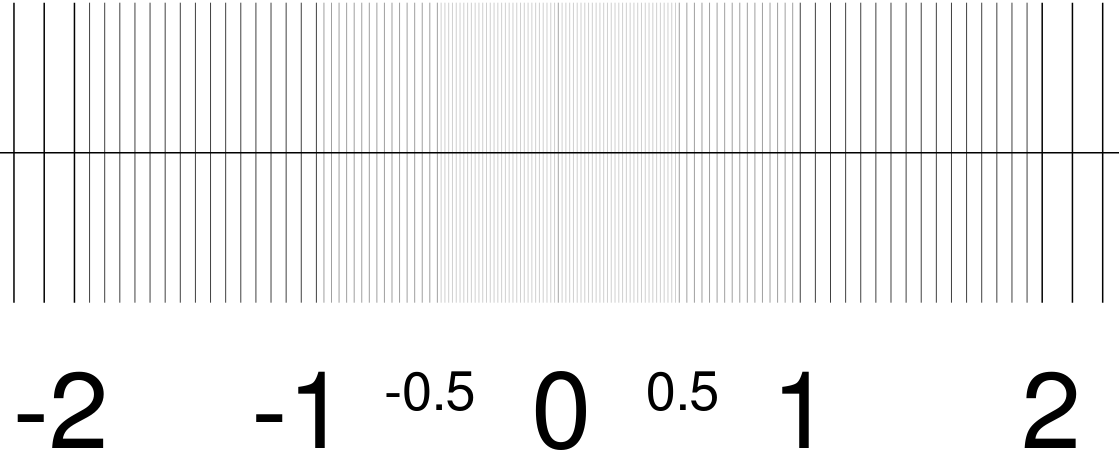
\includegraphics[width=\textwidth]{floating_point_distribution}
%     \centering
%     \caption{Floating point $\left(-1\right)^S\left(1.d_{1}d_{2}d_{3} d_{4}\right)_2\times 2^{\left(e_{1}e_{2} e_{3}\right)_2-3}$ distribution.}
%     \label{img:floatingpointdistribution}
% \end{figure}
% \FloatBarrier

% \subsubsection{Calculation of $\Lambda$}
% \label{subsubsec:calLambda}
% The snapping mechanism uses input $\lambda$ to calculate $\Lambda$. For $n \in \mathbb{Z} $, $\Lambda=2^{n}$ is the smallest power of two greater than or equal to $\lambda$, i.e., $2^{n-1} < \lambda \leq 2^{n}$.

% We can represent $\lambda$ in IEEE 754 floating-point (cf.~\autoref{subsubsec:floatingPoint}) as follows:

% \[ \lambda = (-1)^0 \left(1.d_{1} \hdots d_{52}\right)_2 \times 2^{\left(e_1 \hdots e_{11}\right)_2-1023}. \]

% The calculation of $\Lambda$ can be divided into two cases: (1) $\lambda=2^{n}$ for $n \in \mathbb{Z} $, which requires $\left(d_i\right)_{i \in \left[52\right]} = 0$; (2) $2^{n-1}<\lambda<2^{n}$ for $n \in \mathbb{Z} $. For the first case, we can get $\Lambda\gets \lambda$ since $\lambda=2^{n}$ is already a power of two. For the second case, we can calculate $\Lambda$ by increasing the exponent of $\lambda$ by $1$ and setting all its significant bits $\left(d_i\right)_{i \in \left[52\right]} $ to $0$.

% In summary we have

% \begin{equation}
%     \Lambda =
%     \begin{cases}
%         \lambda                                                                           & \text{ if for } i \in \left[52\right] \text{, } \forall i: d_i = 0    \\
%         \left(1.\overline{0}\right)_2 \times 2^{\left(e_1 \hdots e_{11}\right) _2-1023+1} & \text{ if for } i \in \left[52\right] \text{, } \exists i: d_i \neq 0
%     \end{cases}
% \end{equation}

% \subsubsection{Rounding $x$ to the nearest multiple of $\Lambda=2^n$}
% \label{subsubsec:roundX2Lambda}

% We represent $x$ in IEEE 754 floating-point (cf.~\autoref{subsubsec:floatingPoint}) as follows:
% \[ x = \left(-1\right)^S \left(1.d_{1} \hdots d_{52}\right)_2 \times 2^{\left(e_1 \hdots e_{11}\right)_2-1023}. \]

% $\lfloor x \rceil_{\Lambda}$ is done in three steps:
% \begin{enumerate}
%     \item $x^{\prime} = \frac{x}{\Lambda}=x\cdot 2^{-n}$,
%     \item $x^{\prime\prime}=\left\lfloor x^{\prime}\right\rceil $,
%     \item $\lfloor x \rceil_{\Lambda} = x^{\prime\prime} \cdot   \Lambda  =x\cdot 2^{n}$,
% \end{enumerate}
% where $\left\lfloor \cdot \right\rceil$ rounds the input to the nearest integer.
% % \paragraph{1. $x^{\prime} = \frac{x}{\Lambda}$}

% % We represent $x$ in IEEE 754 floating-point (cf.~\autoref{subsubsec:floatingPoint}) as follows:
% % \[ x = \left(-1\right)^S \left(1.d_{1} \hdots d_{52}\right)_2 \times 2^{\left(e_1 \hdots e_{11}\right)_2-1023}. \]
% % Since $\Lambda=2^n$ is a power of two, the division $\frac{x}{\Lambda}$ can be performed by substracting $n$ from the exponent of $x$ and we get:
% % \[ x^{\prime} = \left(-1\right)^S \left(1.d_{1} \hdots d_{52}\right)_2 \times 2^{\left(e_1 \hdots e_{11}\right)_2-1023-n}. \]

% The first step ($x^{\prime} = \frac{x}{\Lambda}$) and last step ($\lfloor x \rceil_{\Lambda} =   x^{\prime\prime} \cdot \Lambda $) are calculated by manipulating (substraction or addition) the exponent of $x$ and $x^{\prime\prime}$. Note that one exception is when $x=0$ or $x^{\prime\prime}=0$, because for floating-point number $0=\left(-1\right) ^0 (1.\overline{0})_2\times 2^{\left(0000000000\right)_2-1023 }$, $0\times 2^n\neq \left(-1\right) ^0 (1.\overline{0})_2\times 2^{\left(0000000000\right)_2-1023+n }$ as discussed in~\cite{IEEE754_2019}.

% \paragraph{Calculate $x^{\prime\prime}=\left\lfloor x^{\prime}\right\rceil $ }
% \label{para:roundX2Int}

% Suppose $x^{\prime} = \left(-1\right)^S \left(1.d_{1} \hdots d_{52}\right)_2 \times 2^{\left(e_1 \hdots e_{11}\right)_2-1023-n}$. Let $y=\left(e_1 \hdots e_{11}\right)_2-1023-n$, and we have
% \[ x^{\prime} = \left(-1\right)^S \left(1.d_{1} \hdots d_{52}\right)_2 \times 2^{y}.\]
% The calculation of $x^{\prime\prime}=\left\lfloor x^{\prime}\right\rceil $ is categorized in five cases depending on the value of unbiased exponent $y$.

% \textbf{Case 1: $y \geq 52$}\\
% When the biased exponent $y$ is greater than or equal to $52$, $x^{\prime}$ is an integer~\cite{IEEE754_2019}. Then, we have $ x^{\prime\prime} = \left(-1\right) ^S \left(1.d_1 \dots d_{52}\right)_2 \times 2^{y}$.

% \textbf{Case 2: $y =0$}\\
% When $y =0$, we have $ x^{\prime}= (-1)^S (1.d_1 d_2 \hdots d_{52})_2 \times 2^{0} $.
% The rounding result $x^{\prime\prime}$ depends on $d_1$: $x^{\prime\prime}=\left(-1\right)^{S}\times 2^0$ if $d_1=0$, or $x^{\prime\prime}=\left(-1\right)^{S}\times 2^{1}$ if $d_1=1$.
% Therefore, we have $x^{\prime\prime} = \left(-1\right)^S \left(1.\overline{0}\right) _2 \times 2^{d_{1}}$.

% \textbf{Case 3: $y \in \{1, \hdots, 51\}$}\\
% We represent $x^{\prime}$ by right-shifting the radix point $y$ times,and removing the biased exponent $y$:

% \[ x^{\prime} = \left(-1\right) ^S \left(1d_1 \hdots d_{y}.d_{y+1} \hdots d_{52}\right)_2 .\]

% Note that bits $\left(1d_{1}\ldots d_{y}\right)_2 $ are the integer part and bits $\left(.d_{y+1}\ldots d_{52}\right)_2 $ are the fractional part. We have $\left(.d_{y+1}\right)_2 =0.5 $ when $d_{y+1} = 1$, and $\left(.d_{y+1}\right)_2 =0$ when $d_{y+1} = 0$. Therefore, rounding $x^{\prime}$ to the nearest integer means rounding up if $d_{y+1} = 1$, or keeping the integer part unchanged if $d_{y+1} = 0$. In both cases, all bits in the fractional part are set to zeros. \CHANGED{An edge case is when $\left(d_{i}\right)_{i \in \left[y\right]} =1$ and $d_{y+1}=1$, as $\left(d_{i}\right)_{i \in \left[y\right]}=0$ after rounding up}. Therefore, we have to round $x^{\prime}$ by increasing the exponent $y$ by one and setting all bits of the significant to zero.

% In summary we have three subcases that are summarized below:
% \begin{equation}
%     x^{\prime\prime}=
%     \begin{cases}
%         \left(-1\right) ^S \left(1.d^{\prime}_1 \hdots d^{\prime}_y \overline{0}\right)_2 \times 2^{y}, & \text{ if } d_{y+1} = 1 \text{ and } \text{for } i \in \left[y\right] \text{, } \exists i: d_i = 0 \\
%         \left(-1\right)^S \left(1.\overline{0}\right) _2 \times 2^{y+1},                                & \text{ if } d_{y+1} = 1 \text{ and } \text{for } i \in \left[y\right] \text{, } \forall i: d_i = 1 \\
%         \left(-1\right)^S \left(1.d_1 \hdots d_y \overline{0}\right) _2 \times 2^{y},                   & \text{ if } d_{y+1} = 0
%     \end{cases}
% \end{equation}
% where $\left(d_1^{\prime}\ldots d_y^{\prime}\right)_2 =\left(d_1\ldots d_y\right)_2 +1 $.

% \textbf{Case 4: $y = -1$}\\
% When $y=-1$, we have $x^{\prime}= (-1)^S (0.1d_1 d_2 \hdots d_{51})_2$.
% Since the digit after the radix point is always $1$, $x^{\prime}$ is round to $\left(-1\right)^{S}\times 2^0$. Therefore, $x^{\prime\prime}$ can be represented in IEEE 754 floating-point (cf.~\autoref{subsubsec:floatingPoint}) as follows:
% \[  x^{\prime\prime}=\left(-1\right)^{S}\left(1.\overline{0}\right)_2 \times 2^{\left(01111111111\right)_2-1023 } .\]

% \textbf{Case 5: $y < -1$}\\
% When $y < -1$, we have $x^{\prime}= (-1)^S (0.01d_1 d_2 \hdots d_{50})_2$.
% Since the digit after the radix point is $0$, $x^{\prime}$ is always rounded to $0$. We set $x^{\prime\prime}\gets\pm 0$ which can be represented in IEEE 754 floating-point (cf.~\autoref{subsubsec:floatingPoint}) as follows:
% \[ +0 = (-1)^0 (1.\overline{0})_2\times 2^{\left(0000000000\right)_2-1023 } ,\]
% \[ -0 = (-1)^1 (1.\overline{0})_2\times 2^{\left(0000000000\right)_2-1023 } .\]


% \paragraph{3. Multiply $x^{\prime\prime}$ by $\Lambda$}

% In floating-point arithmetic, multiply $x^{\prime\prime}$ by $\Lambda=2^n$ can be calculated by adding $n$ to the exponent of $x^{\prime\prime}$.

% One exception is when $x^{\prime\prime}=\pm0$ since $\left(\pm0\right)  \times 2^n= (-1)^S (1.\overline{0})_2\times 2^{\left(0000000000\right)_2-1023+n }$ doesn't represent the values $\pm 0$ as~\cite{IEEE754_2019}.


\section{Integer-Scaling Mechanism}
\label{sec:integerScalingMechanism}
Google Differential Privacy Team~\cite{googleDP2019} proposed a differentially private algorithm that can achieve similar DP protection as Laplace mechanism (cf.~\autoref{def:laplaceMechanism}) or Gaussian mechanism (cf.~\autoref{def:gaussianMechanism}) by re-scaling a discrete random variable to simulate the continuous random variable, which is defined as follows:
\begin{equation}
    \begin{split}
        M_{IS}\left(f\left(D\right),r, \varepsilon, \delta \right)=f_r\left(D\right) +ir.
    \end{split}
\end{equation}

% where $i\sim DLap\left(\frac{\Delta_r}{r \epsilon}\right) $ is re-scaled by the resolution parameter $r=2^k$ (with $k \in \left[-1021,970\right] $) to simulate continuous Laplace noise. $\Delta_r =\Delta_1 ^{f}+r$
where discrete random variable $i $ is re-scaled by the resolution parameter $r=2^k$ (for $k \in \left[-1022,970\right] $) to simulate a continuous random variable.
;Function $f_r\left(D\right)\in\mathbb{D} $ rounds the output of query function $f\left(D\right)\in\mathbb{R} $ to the nearest multiple of $r$.
$r$ determines the scale of the continuous random variable $ir$ is simulating and is predefined.
$\varepsilon, \delta$ are the parameters that define the level of differential privacy guarantee.

\textbf{Main Idea. } Assume $f_r\left(D\right) +ir$ satisfy $\left(\varepsilon, \delta\right) $-DP under real number arithmetic, if $f_r\left(D\right) +ir$ can be computed \textit{precisely} under floating-point arithmetic, then we can conclude that $f_r\left(D\right) +ir$ can also satisfies $\left(\varepsilon, \delta\right) $-DP under floating-point arithmetic. \textit{Precisely} indicates that the real numbers are represented as floating numbers without precision loss, and the arithmetic operations of these real numbers yield the exactly same result as when these real numbers are represented as floating-point numbers.
If integer $\left\lvert i\right\rvert \leq2^{52}$ (or $\Pr\left(\left\lvert i>2^{52}\right\rvert \right) $ is small enough to be ignored), then we have $    \left\lvert ir\right\rvert  \leq 2^{1022}$. Therefore, $ir$ can be represented precisely as a floating-point number by adding $k$ to the exponent of $i$. Further, by choosing $r$ and limiting $\left\lvert f\left(D\right)\right\rvert< 2^{52}r  $, we can guarantee that $f_r\left(D\right) $ and $f_r\left(D\right)+ir$ can be represented precisely as a floating-point number.
Finally, it proved that $f_r\left(D\right) +ir$ satisfies $\left(\varepsilon, \delta\right)$-DP under floating-point implementation.

% Note that in original work~\cite{googleDP2019}, the sampling algorithms of integer $i$ is called secure noise generation (SNG).

% % The main idea of integer-scaling mechanism is as follows: We first prove that $M_{IS}\left(f\left(D\right),r\right)$ under exact real number arithemtic satisfy differential privacy. Then, we implement $M_{IS}\left(f\left(D\right),r\right)$ under floating-point number arithmetic such that the difference to exact real number arithmetic is negligible. Finally, we prove that $M_{IS}\left(f\left(D\right),r\right)$ under floating-point number arithmetic also satisfy differential privacy. 

% The key challenge thereby is to calculate $M_{IS}\left(f\left(D\right),r\right)$ under floating-point arithmetic \textit{precisely} as if under real number arithmetic. \textit{Precisely} indicates to represent real numbers as floating numbers without precision loss, and the arithmetic operations of those real numbers yield the same result when these real numbers are represented as floating-point numbers. In this way, $M_{IS}\left(f\left(D\right),r\right)$ is immune to the attack described in Mironov's work~\cite{mironov2012significance}. 
% By sampling integer $i$ from differential distribution, the integer-scaling mechanism can achieve similar DP-guarantee as Laplace mechanism (cf.~\autoref{def:laplaceMechanism}) or Gaussian mechanism (cf.~\autoref{def:gaussianMechanism}). 


% % \TODO{ origin paper https://github.com/google/differential-privacy/blob/main/common_docs/Secure_Noise_Generation.pdf (page 3) about represent operation in floating-point contains errors}\\

% % \subsection{Framework for Integer-scaling Mechanism}
% % \label{subsec:FrameworkIntegerScalingMechanism}
% % In this part, we describe how to implement $M_{IS}\left(f\left(D\right),r\right)$ \textit{exactly} under floating-point arithmetic inspired by the work~\cite{googleDP2019}. Recall a floating-point number $d$ can be represented in IEEE 754 floating-point (cf.~\autoref{subsubsec:floatingPoint}) as follows:
% % \[d_{IEEE-754}=\left(-1\right)^S \left(1.d_{1}\ldots d_{52}\right)_{2}\times2^{\left(e_1\ldots e_{11}\right)_2 -1023},\]
% % where $\left(d_{1},\ldots ,d_{52}\right) \in \left\{0,1\right\}^{52}  $ are the significant bits, $\left(e_1\ldots e_{11}\right)\in\left\{0,1\right\}^{11} $ are the biased exponent bits, and $S\in\left\{0,1\right\} $ is the sign bit.

% % $d$ can be reformulated by right-shifting the radix point for $52$ times, and substracting $52$ from the exponent as follows:
% % \[d_{Rshift\left(52\right) }=\left(-1\right)^S \left(1 \times 2^{52}+\left( d_{1}\ldots d_{52}.\right)_{2}\right)\times2^{\left(e_1\ldots e_{11}\right)_2 -1023-52}.\]
% % We use the above $d_{Rshift\left(52\right) }$ floating-point number format to represent the terms of $M_{IS}\left(f\left(D\right),r\right)$.

% % Let $i=\left(i_1\ldots i_{52}\right)_2$ with $\left(i_1,\ldots ,i_{52}\right)\in \left\{0,1\right\}^{52}$, $t=\left(t_1\ldots t_{52}\right)_2$ with $\left(t_1,\ldots ,t_{52}\right)\in \left\{0,1\right\}^{52}$, and $r=2^{\left(r_{e_{1}}\ldots r_{e_{11}}\right)_2-1023-52}$ with $\left(r_{e_{1}},\ldots ,r_{e_{11}}\right)\in \left\{0,1\right\}^{11} $. Let $f_r\left(D\right)=t r$, where $t r$ is the nearest multiple of $r$ to $f\left(D\right)$.

% % Then, $M_{IS}\left(f\left(D\right),r\right)$ can be represented with $d_{Rshift\left(52\right) }$ floating-point number format as follows:

% % \begin{equation}
% %     \begin{split}
% %         M_{IS}\left(f\left(D\right),r\right) & =f_r\left(D\right) +ir \\
% %         & =tr+ir\\
% %         & =\left(2^{52}+t\right)\cdot r+ \left(2^{52}+i\right)\cdot r-2^{52}\cdot r-2^{52}\cdot r.\\
% %     \end{split}
% % \end{equation}

% % Note that
% % \begin{equation}
% %     \begin{split}
% %         \left(2^{52}+t\right)\cdot r&=\left(2^{52}+t\right)\cdot 2^{\left(r_{e_{1}}\ldots r_{e_{11}}\right)_2-1023-52}\\
% %         &=\left(2^{52}+\left(t_1\ldots t_{52}\right)_2 \right)\cdot 2^{\left(r_{e_{1}}\ldots r_{e_{11}}\right)_2-1023-52}\\
% %         &=\left(1.t_1\ldots t_{52}\right)_2 \cdot 2^{\left(r_{e_{1}}\ldots r_{e_{11}}\right)_2-1023}. \\
% %     \end{split}
% % \end{equation}

% % Therefore, $\left(2^{52}+t\right)\cdot r$, $\left(2^{52}+i\right)\cdot r$ and $2^{52}\cdot r=1\cdot 2^{\left(r_{e{_1}}\ldots r_{e_{11}}\right)_2-1023}$ can be represented exactly as floating-point numbers without rounding or truncation. In other words, we calculate the terms of $M_{IS}\left(f\left(D\right),r\right)$ exactly under floating-point arithmetic.

% % In summary, the calculation of $M_{IS}\left(f\left(D\right),r\right)$ consists of three steps:
% % \begin{enumerate}
% %     \item Choose a resolution parameter $r=2^k$, where $k \in \left[-1022 \ldots 971\right] $.
% %     \item Sample $i$ from $Sampler\left(\epsilon ,\delta ,r,\Delta _r^{}\right) $, which guarantees that $\text{Pr}\left[\left\lvert i\right\rvert > 2^{52}\right] <\frac{1}{e^{\left(1000\right)}} $.
% %     \item Calculate $f_r\left(D\right) +ir$ under floating-point arithmetic.
% % \end{enumerate}

% % \TODO{prove about $\text{Pr}\left[\left\lvert i\right\rvert > 2^{52}\right] <\frac{1}{e^{\left(1000\right)}} $ or better bound}

% % Step $1,2$ guarantee that the scaled integer $ir$ can be represented exactly as floating-point numbers with very high probability (fails with very low probability $p<\frac{1}{e^{\left(1000\right)}}$). $i$ is an integer generated by $Sampler\left(\epsilon ,\delta ,r,\Delta _r\right) $ that corresponds to a probability distribution, where $\epsilon$, $\delta$ are the parameters that controls the privacy protection level, and $\Delta _r$ is the sensitivity of $f_r\left(D\right)$. Similar to the sensitivity definition of $f\left(D\right) $ (cf.~\autoref{def:sensitivity}), the sensitivity of $f_r\left(D\right)$ is defined as $\Delta_r =\max _{D,D^{\prime}}\left\lVert f_r\left(D\right) -f_r\left(D^{\prime}\right) \right\rVert $, where $D$ and $D^{\prime}$ are neighboring databases.

\subsection{Integer-Scaling Laplace Mechanism}
\label{subsec:ISLap}
In this section, we describe the integer-scaling Laplace mechanism~\cite{googleDP2019} and modifying the corresponding sampling algorithms.

The integer-scaling Laplace mechanism~\cite{googleDP2019} is defined as:
\begin{equation}
    \begin{split}
        M_{ISLap}\left(f\left(D\right),r,\Delta _r,\varepsilon\right)=f_r\left(D\right) +ir,
    \end{split}
\end{equation}

where $r$ is the resolution parameter that controls the scale of the simulated continuous Laplace random variable $ir$, integer $i \sim DLap\left(t=\frac{\Delta_r}{r\varepsilon}\right) $ (cf.~\autoref{def:DiscreteLaplaceDistribution}), $\Delta _r=r+\Delta^f_1$, and $\Delta^f_1$ is the sensitivity (cf.~\autoref{def:sensitivity}) of $f\left(D\right)$.

\begin{theorem}[\cite{googleDP2019}]
    The integer-scaling Laplace mechanism $M_{ISLap}\left(f\left(D\right),r,\Delta _r,\varepsilon\right)$ satisfies $\varepsilon$-DP for query function $f$.
\end{theorem}

We found three discrete Laplace sampling algorithms~\cite{eigner2014differentially,googleDP2019,canonne2020discrete } that can be used in integer-scaling Laplace mechanism.
We only describe and modify the discrete Laplace sampling algorithm in work~\cite{googleDP2019} that first generates a geometric random variable $x$ with a binary based geometric sampling algorithm and convert $x$ to a discrete Laplace random variable.
% As the discrete Laplace distribution can be generate by reflecting the geometric distribution across $y$-axis, we can first sample a geometric random variable and transform it into a discrete Laplace random variable. $r$ is the smallest power of $2$ exceeding $ \frac{\Delta }{2^c\epsilon}$, $\varepsilon$ controls the differential privacy protection level (cf.~\autoref{def:laplaceMechanism}), and $c\in \left\{10, 11,\ldots, 45\right\} $ is a predefined parameter that controls the degree of discretization and accuracy of $M_{ISLap}\left(f\left(D\right),r,\varepsilon,\Delta _r\right)$.\\

% % \TODO{explain, how to choose $c$ in practice, influence on accuracy...}\\


% \TODO{DP prove, properties.}

% In the following part, we introduce the sampling algorithms for geometric random variables and two-side geometric random variables based on work~\cite{googleDP2019}.

% \subsubsection{Geometric Distribution Sampling}
% \label{subsubsec:geometricExpBinarySearch}

\paragraph{Binary Search Based Geometric Sampling Algorithm}
\label{para:BinarySearchBasedGeometricSamplingAlgorithm}

\autoref{algo:GeometricExpBinarySearch} is a modification of the binary search based geometric sampling algorithm from the work~\cite{googleDP2019GitHub} that samples a positive integer $x$ from a geometric distribution $Geo\left(x\,|\,p=1-e^{-\lambda}\right)=\left(1-p\right)^{x-1}\cdot p $.

\textbf{Sampling Interval of $x$.}
Let's first define the sampling interval of geometric random variable $x$ and $\lambda$.
We sample random variable $x \in \left[1, 2^{52}\right] $.
In original work~\cite{googleDP2019GitHub}, the sampling interval for $x$ is $ \left[1, 2^{63}-1\right]$. We limit the sampling interval of $x$ to $\left[1, 2^{52}\right]$ because each integer in  $\left[1, 2^{52}\right]$ can be represented exactly as a floating-point number.

% $x\cdot r=x \cdot 2^k$ can be calculated precisely under floating-point arithmetic without additional operations as follows:

% \begin{equation}
%     \begin{split}
%         1 \cdot 2^k\leq & x \cdot 2^k  \leq Int_{max53} \cdot 2^{k}\\
%         2^k\leq &x \cdot 2^k  \leq 2^{k+52}
%     \end{split}
% \end{equation}

% Because $k \in \left[-1022,970\right]$, we have $k+52\in \left[-970,1022\right] $ and which indicates that $x\cdot r =x\cdot 2^k$ is a valid double-precision floating-point number (cf.~\autoref{subsubsec:floatingPoint}).

% As discussed in~\autoref{subsec:FrameworkIntegerScalingMechanism}, the random variable integer $x\in \left\{0,1\right\} ^{52}$ and $x\leq \left(\overline{1}_{\left(52\right) }\right)_2 $. Therefore, we choose $\left(0\ldots Int_{max52}\right] $ as the sample interval.

\textbf{Choice of $\lambda$. }
Then, we set a reasonable value range for parameter $\lambda$ (original work~\cite{googleDP2019} requires $\lambda > 2^{-59}$).
For the geometric distribution's CDF: $\Pr\left(x\leq X \right) =1-\left(1-p\right)^X $ with $X=2^{52}$, we have
\begin{equation}
    \text{CDF}: \text{Pr}\left(x \leq 2^{52}\right)=
    1-e^{-\lambda\cdot 2^{52} }=
    \begin{cases}
        0.\overline{9}_{\left(27\right) }8396\ldots & \text{ for }\lambda=2^{-48} \\
        0.\overline{9}_{\left(13\right) }8734\ldots & \text{ for }\lambda=2^{-49} \\
    \end{cases}
\end{equation}

We require $\lambda\geq 2^{-48}$ which means that the probability \autoref{algo:GeometricExpBinarySearch} fails (to generate $x>2^{52}$) is $ 1- 0.\overline{9}_{\left(27\right) }8396 \approx 2^{-92}$.
% % The support of the geometric distribution $Geo\left(p\right) $ is $supp\left(Geo\left(p\right) \right)=\left\{z \in \mathbb{Z} \,|\, z>0\right\}  $. However, since we can only sample integers from interval $\left[1, Int_{max52}-1\right] $, $\text{Pr}\left(x \leq Int_{max53}\right)$ should be close to $1$. Thus, we set $\lambda\geq2^{-49}$ to ensure $\text{Pr}\left(x \leq Int_{max53}\right)\geq 0.\overline{9}_{\left(6\right) }8875\ldots$.

\textbf{Algorithm Description. }
\autoref{algo:GeometricExpBinarySearch} samples a geometric random variable $x$ by splitting the sampling interval into two subintervals with the almost same cumulative probability, then one subinterval is chosen at random and the other is discard. This sampling interval splitting and choosing process is repeated until and the remaining sampling interval only contains one value which is the geometric random variable $x$ we are looking for. In original work~\cite{googleDP2019}, the sampling algorithm additional checks if the generated random variable exceed the sampling interval $\left[0,  2^{63}-1\right] $, that is not necessary in our case because we set $\lambda>2^{-48}$ such that it happens with low probability $p \approx 2^{-92}$.

% We replace the $WHILE$ loop (line 2) of original work to $FOR$ loop because the number of loop iterations must be determined for MPC computations. 
In Line $1$, we set the initial sampling interval to $\left(0,2^{52}\right] $.
In Line $ 3$, the sampling interval $\left(L\ldots R\right] $ is first splitted with function $\text{Split}\left(L,R,\lambda\right)=L-\frac{\ln\left(0.5\right)+\ln\left(1+e^{-\lambda\left(R-L\right) }\right) }{\lambda}$ into two subintervals ($\left(L\ldots M\right] $ and $\left(M\ldots R\right] $), such that they have approximately equal cumulative probability (i.e., $Pr\left(Geo\left(L<x\leq M\right) \right) \approx Pr \left(Geo\left(M  \leq x  < R\right) \right)  $).
    % More specifically, function $\text{Split}\left(L,R,\lambda\right)=L-\frac{\ln\left(0.5\right)+\ln\left(1+e^{-\lambda\left(R-L\right) }\right) }{\lambda}$ calculates the middle point $M$ of sampling interval $\left(L\ldots R\right] $ such that for $Geo\left(p=1-e^{-\lambda}\right) $'s probability mass function: $\text{Pr}\left(L< x \leq M \, | \, L < x\leq R\right)\approx \frac{1}{2}$.
    Line $4-7$ ensure that the middle point $M$ lies in interval $(L\ldots R]$ (or relocate $M$ to interval $(L\ldots R]$ otherwise).
    Line $8$ calculates the cumulative probability proportion $Q$ between $\left(L\ldots M\right] $ and $\left(M\ldots R\right] $ with function $\text{Proportion}\left(L,R,M,\lambda\right)=\frac{e^{-\lambda\left(M-L\right) }-1}{e^{-\lambda\left(R-L\right) }-1} $.
    In line $9-13$, we randomly choose one interval based on the comparison result of the generated uniform variable $U$ (cf.~\autoref{subsubsec:generationUStar}) and $Q$.
    % Specifically, suppose $\text{Pr}\left(L< x \leq M \right)=l$ and $\text{Pr}\left(M< x \leq R \right)=r$, we have $Q=\frac{l}{l+r}$. 
    If $U \leq Q$, we choose $\left(L\ldots M\right] $ as the next sampling interval, $\left(M\ldots R\right] $ otherwise. In other words, the probability that an interval is chosen is proportional to its cumulative probability.
    The whole process is repeated (less than $52$ times) until the remaining interval contains only one value (Line $2$). Finally, we set $x\gets R$, where $x\sim Geo\left(p=1-e^{-\lambda}\right)$ (details can be found in \autoref{sec:additionalProof}).


    % Note that $Q$ should be approximate to $\frac{1}{2}$ as discussed in function $\operatorname{Split}\left(L,R,\lambda\right)$. 

    % Then, based on the comparison result of $Q$ and uniform floating-point number $U^{*}\in\mathbb{D}  \cap\left(0,1\right) $, either interval $\left(L\ldots M\right] $ or interval $\left(M\ldots R\right] $ will be chosen. 



    % Note that one implicit assumption of $Algo^{GeoExpBinarySearch}\left(\lambda\right) $ is that the uniform random variable $U^{*} \leq 1-e^{-\lambda Int_{max52}}$ or $1-e^{-\lambda Int_{max52}} \approx 1$. For example, suppose $\lambda$ is a very small value such than $\lambda \cdot Int_{max52}=4$, then we have CDF: $\text{Pr}\left(x \leq Int_{max52}\right)=1-e^{-4}=0.9816\ldots$ which means the cumulative probability of the sampling interval $\left(0\ldots Int_{max52}\right] $ is $0.9816\ldots$ and random variables $x> Int_{max52}$ (can't be generated by the algorithm) has probability $1-0.9816\ldots$.

    \begin{algorithm}[tbh!]
        \centering
        \fbox{
            \pseudocode[space=none, syntaxhighlight=auto, addkeywords={Algorithm, Input, Output, IF,TO,RETURN, FOR, ELSE IF, ELSE, WHILE},linenumbering, skipfirstln, head=\textbf{Algorithm: $Algo^{GeoExpBinarySearch}\left(\lambda\right) $}]{
                \textbf{Input: $\lambda$} \pcskipln \\
                \textbf{Output: $x\sim Geo\left(p=1-e^{-\lambda}\right) $} \\
                % \text{$U^{*} \gets Algo^{RandFloat1}$}\\
                % \text{IF $U^{*}>1-e^{-\lambda Int_{max52}}$.}\\
                % \text{\t\t RETURN $Int_{max52}$} \\
                \text{$L \gets 0$, $R \gets 2^{52}$}\\
                \text{WHILE $L+1<R$}\\
                \text{\t\t $M\gets \text{Split}\left(L,R,\lambda\right) $}\\
                \text{\t\t IF $M\leq L$}\\
                \text{\t\t \t\t $M\gets L+1$}\\
                \text{\t\t ELSE IF $M \geq R$}\\
                \text{\t\t \t\t $M\gets R-1$}\\
                \text{\t\t $Q\gets \text{Proportion}\left(L,R,M,\lambda\right) $}\\
                \text{\t\t $U \gets Algo^{RandFloat1}$}\\
                \text{\t\t IF $U\leq Q$}\\
                \text{\t\t \t\t $R\gets M$ }\\
                \text{\t\t ELSE }\\
                \text{\t\t \t\t $L\gets M$}\\
                \text{RETURN $x\gets R$}
            }}
        \caption{Modified algorithm for sampling from geometric distribution $Geo\left(p=1-e^{-\lambda}\right) $.}
        \label{algo:GeometricExpBinarySearch}
    \end{algorithm}
    \FloatBarrier


    \paragraph{Two-Side Geometric Sampling Algorithm}
    \label{para:TwoSideGeometricSamplingAlgorithm}
    In this part, we describe how to transform $x \sim Geo\left(p=1-e^{-\lambda}\right) $ to $i\sim DLap\left(t=\frac{1}{\lambda}\right) $ based on the work~\cite{googleDP2019}.

    \textbf{Algorithm Description. }
    Recall that two-side geometric distribution (also known as discrete Laplace distribution) can be generated by reflecting a geometric distribution across the $y$-axis (cf. \autoref{def:DiscreteLaplaceDistribution}).
    \autoref{algo:TwoSideGeometric} generates a discrete Laplace random variable $i=s\cdot g$ with this method. We replace the $WHILE$ loop (line 1) in original work into a $FOR$ loop because the MPC computation needs to determine the number of $FOR$ loops ahead of time.
    In line $4$, we discard the case $s\cdot g =-0$, otherwise $0$ would be returned with twice probability as in discrete Laplace distribution.
    In line $5$, we output the correct discrete Laplace random variable $i$.
    In line $6$, the algorithm fails to generate discrete random variable in $ITER$ loops and output $0$.

    \begin{algorithm}[tbh!]
        \centering
        \fbox{
            \pseudocode[space=none, syntaxhighlight=auto, addkeywords={Algorithm, Input, Output, IF,TO,RETURN, FOR, ELSE IF, ELSE, WHILE, AND},linenumbering, skipfirstln, head=\textbf{Algorithm: $Algo^{TwoSideGeo}\left(t\right) $}]{
                \textbf{Input: $t$} \pcskipln \\
                \textbf{Output: $i\sim DLap\left(t\right) $} \\
                \text{FOR $i\gets 1$ TO $ITER$}\\
                \text{\t\t $g \gets Algo^{GeoExpBinarySearch}\left(\lambda=\frac{1}{t}\right)$}\\
                \text{\t\t $s\gets 2 \cdot Bern\left(0.5\right)-1$}\\
                \text{\t\t IF $\lnot \left(s== -1 \land g== 0\right) $}\\
                \text{\t\t \t\t RETURN $i \gets s\cdot g$ // success}\\
                \text{RETURN $i \gets 0$ // failure}
            }}
        \caption{Modified algorithm for sampling $i\sim DLap\left(t\right) $.}
        \label{algo:TwoSideGeometric}
    \end{algorithm}
    \FloatBarrier

    \textbf{Algorithm Fail Probaility Estimation. }
    Suppose $A_i$ is an event that \autoref{algo:TwoSideGeometric} fails when $ITER=i$.
    Since each iteration is independent, we estimate the $Pr\left(A_{ITER}\right)$ as follows:
    \begin{equation}
        \begin{split}
            Pr\left(A_{ITER}\right) & = \Pi _{i=1}^{ITER}\left(Pr\left(A_1\right) \right) \\
            &= \Pi _{i=1}^{ITER} \left(Pr\left(s==-1\right)\cdot  Pr\left(g==0\right) \right)\\
            &=       \Pi _{i=1}^{ITER} \left(Pr\left(0\gets Bern\left(0.5\right) \right)\cdot Pr\left(0\gets Geo\left(\frac{1}{t}\right) \right)  \right)                   \\
            &= \Pi _{i=1}^{ITER} \frac{1}{2}  \left(1-e^{-\lambda}\right) \\
            &= \frac{1}{2^{ITER}}  \left(1-e^{-\lambda}\right)^{ITER}.
        \end{split}
    \end{equation}

    To guarantee that $Pr\left(A_{ITER}\right)<2^{-40}$, we have $ITER = 6$ for $\lambda = 0.01$.




    \subsection{Integer-Scaling Gaussian Mechanism}
    \label{subsec:IntegerScalingGaussianMechanism}
    In this section, we describe the integer-scaling Gaussian mechanism $M_{ISGauss}\left(f\left(D\right),r,\Delta_r,\varepsilon,\delta\right)=f_r\left(D\right) +ir$ in work~\cite{googleDP2019}.
    Specifically, $M_{ISGauss}\left(f\left(D\right),r,\Delta_r,\varepsilon,\delta\right)$ uses a symmetrical binomial random variable $i\sim SymmBino\left(n,p=0.5\right) $ (cf.~\autoref{def:binomialdistribution}) to simulate the continuous Gaussian random variable $i_{Gau}\sim \mathcal{N} \left(\mu=0,\sigma^2=\frac{2 \ln\left(1.25/\sigma \cdot \left(\Delta_1^f\right)^2 \right) }{\varepsilon^2}\right) $. The closeness between the symmetrical and Guassian distribution depends on $n$, i.e., a larger $n$ indicates a better approximation effect. $n$ can be estimate with $varepsilon$, $delta$ (cf.~\autoref{ImproveGaussianMechanism}) and $\sqrt{n} $ is guaranteed to be in $\left[2^{56},2^{57}\right] $. Note that in the following part, we use the square root of $n$ instead of $n$ as $n$ is too large to be represented as a 64-bit floating-point number.

    \begin{theorem}[\cite{googleDP2019}]
        The integer-scaling Gaussian mechanism $M_{ISGauss}\left(f\left(D\right),r,\Delta_r,\varepsilon,\delta\right)$ satisfies $ \left(\varepsilon,\delta\right) $-DP for query function $f$.
    \end{theorem}

    % \TODO{explain the parameter of $M_{ISGauss}$, DP-guarantee of $M_{ISGauss}$, add proof missing in original work, }\\
    % where $i$ is sampled from a symmetrical binomial distribution $SymmBino\left(n,p=0.5 \right)$. $M_{ISGauss}\left(f\left(D\right),r,\varepsilon,\sigma,\Delta_r\right)$
    % The binomial distribution $Bino\left(n,p\right)$ is the discrete probability distribution of the number of successes (with probability $p$) in a sequence of $n$ independent experiments.

    % Suppose $x\sim Bino\left(n_x,p\right)$ and $y\sim Bino\left(n_y,p\right)$. We have that $x+y \sim Bino\left(n_x+n_y,p\right)$~\cite[Lemma 4.3]{Devroye1986}. Note that $x$ and $y$ can be generated by independently flipping a coin for $n_x$ and $n_y$ times and counting the numbers of $head$.
    % However, for a very large $n$ (e.g., $n\approx 2^{96}$), this combination method is infeasible. Therefore, a team from Google~\cite{googleDP2019} proposes a rejection based binomial sampling algorithm (cf.~\autoref{algo:SymmetricBinomialLargeN}) that is efficient for large $n$.

    % \TODO{how to modify exactly, origin algorithms, prove}\\
    \paragraph{Symmetrical Binomial Sampling Algorithm}
    \label{para:BinarySearchBasedGeometricSamplingAlgorithm}

    \autoref{algo:SymmetricBinomialLargeN} is an modification of the symmetrical binomial sampling algorithm~\cite{googleDP2019}, that samples $i\sim SymmBino\left(n,p=0.5\right) $ with input $\sqrt{n}\approx 2^{56}$. We modify the original sampling algorithm by replacing the $WHILE$ loop with a $FOR$ loop (line 2), such that it has fixed round of iterations. We also found that when $-\frac{\sqrt{n\ln n}}{2} \leq x \leq \frac{\sqrt{n\ln n}}{2}$, $\tilde{p}\left(x\right)>0$ for $x \in [2^{56},2^{57}]$. Therefore, we replace the $IF$ condition from $\tilde{p}\left(x\right)>0$ (in orignal work) to $\left(-\frac{\sqrt{n\ln n}}{2} \leq x \leq \frac{\sqrt{n\ln n}}{2} \land c==1\right) $ (line 14) that simplifies the construction of MPC protocols.

    % Note that for $n\approx 2^{96}$, $\sqrt{n}=2^{48}$ can be precisely represented as a double-precision floating-point (cf.~\autoref{subsubsec:floatingPoint}) (see \autoref{app:algorithms} for details).

    % % In $Algo^{Binomial}\left(\sqrt{n}\right) $, $Algo^{RandInt}\left(m\right)$~\cite{barker2015recommendation} generates a uniform random integer $l \in \left[0\ldots m\right) $ and $Algo^{Bernoulli}\left(\frac{\tilde{p}\left(i\right)}{f}\right)$ generates a Bernoulli random variable $c\sim Bern\left(p=\frac{\tilde{p}\left(i\right)}{f}\right) $.\\

    \begin{algorithm}[tbh!]
        \centering
        \fbox{
            \pseudocode[space=none, syntaxhighlight=auto, addkeywords={Algorithm, Input, Output, IF,TO,RETURN,AND, FOR, ELSE IF, ELSE, WHILE, TRUE, FALSE},linenumbering, skipfirstln, head=\textbf{Algorithm: $Algo^{SymmetricBinomial}\left(\sqrt{n}\right) $}]{
                \textbf{Input: $\sqrt{n}$} \pcskipln \\
                \textbf{Output: $i\sim SymmBino\left(n,p=0.5\right) $} \\
                \text{$m \gets \left\lfloor \sqrt{2}*\sqrt{n}+1\right\rfloor $}\\
                \text{FOR $j\gets 1$ TO $ITER$ }\\
                \text{\t\t $s \gets Algo^{Geometric\left(0.5 \right) } $}\\
                \text{\t\t $b \gets RandBit\left(1\right) $}\\
                \text{\t\t IF $U^{*}<0.5$}\\
                \text{\t\t \t\t $k \gets s$}\\
                \text{\t\t ELSE}\\
                \text{\t\t \t\t $k \gets -s-1$}\\
                % \text{\t\t $k \gets b\cdot s+\left(1-b\right)\cdot \left(-s-1\right)  $}
                \text{\t\t $l \gets Algo^{RandInt}\left(m\right) $}\\
                \text{\t\t $x\gets km+l$}\\
                % \text{\t\t $\tilde{p}\left(x\right)=\sqrt{\frac{2}{\pi n}} \cdot e^{-\frac{2 x^{2}}{n}} \cdot \left(1-\nu_{n}\right) $, where $\nu_{n}=\frac{0.4 \ln ^{1.5}(n)}{\sqrt{n}}$}\\
                \text{\t\t $\tilde{p}\left(x\right)=\sqrt{\frac{2}{\pi n}} \cdot e^{-\frac{2 x^{2}}{n}} \cdot \left(1-\frac{0.4 \ln ^{1.5}(n)}{\sqrt{n}}\right) $ }\\
                \text{\t\t $f \gets \frac{4}{m\cdot 2^s}$}\\
                \text{\t\t $c \gets Algo^{Bernoulli}\left(\frac{\tilde{p}\left(x\right)}{f}\right) $}\\
                \text{\t\t IF $-\frac{\sqrt{n\ln n}}{2} \leq x \leq \frac{\sqrt{n\ln n}}{2} \land c==1$}\\
                \text{\t\t \t\t RETURN $i\gets x$ // success}\\
                \text{\t\t ELSE}\\
                \text{\t\t \t\t RETURN $i\gets 0$ // failure}
            }}
        \caption{Algorithm for sampling $i\sim SymmBino\left(\sqrt{n} ,p=0.5\right) $.}
        \label{algo:SymmetricBinomialLargeN}
    \end{algorithm}
    \FloatBarrier

    \textbf{Algorithm Fail Probaility Estimation. }
    Suppose $A_i$ is an event that \autoref{algo:SymmetricBinomialLargeN} fails when $ITER=i$.
    Bringmann et al.~\cite{Bringmann2014InternalDE} showed that each iteration has probability $\frac{1}{16} $ to terminate, i.e., $Pr\left(A_1\right)=\frac{15}{16} $.
    Since each iteration is independent, we estimate the $Pr\left(A_{ITER}\right)$ as follows:

    \begin{equation}
        \begin{split}
            Pr\left(A_{ITER}\right) &  =  \Pi _{i=1}^{ITER}\left(Pr\left(A_1\right) \right) \\
            &=\left(\frac{15}{16}\right)^{ITER}
        \end{split}
    \end{equation}

    To guarantee that $Pr\left(A_{ITER}\right)<2^{-40}$, we need at least $ITER\geq \log _\frac{15}{16}\left(2^{-40}\right)\approx 430$.

    \section{Discrete Laplace Mechanism}
    \label{sec:discreteLaplacemechanism}

    In this section, we describe the discrete Laplace mechanism~\cite{chan2012privacy, ghosh2012universally,eigner2014differentially,canonne2020discrete} and present the modified sampling algorithm~\autoref{algo:DiscreteLapCKS}.

    The discrete Laplace mechanism is define as:
    \begin{equation}
        \begin{split}
            M_{DLap}\left(f\left(D\right),r,\varepsilon\right)=f\left(D\right) +Y,
        \end{split}
    \end{equation}
    where query function $f\left(D\right)\in\mathbb{Z} $ and $Y\sim DLap\left(t=\frac{\Delta_1^{f}}{\varepsilon}\right) $.

    \begin{theorem}[\cite{chan2012privacy, ghosh2012universally,eigner2014differentially,canonne2020discrete}]
        The discrete Laplace mechanism $M_{DLap}\left(f\left(D\right),r,\varepsilon\right)$ satisfies $\varepsilon$-DP for query function $f\left(D\right)\in\mathbb{Z} $.
    \end{theorem}

    Except the previous introduced discrete Laplace sampling algorithm (cf.~\autoref{algo:DiscreteLaplaceEigner}), Canonne et al.~\cite{canonne2020discrete} proposed a discrete Laplace sampling algorithm that is based on rejection sampling~\cite{casella2004generalized} technique. The algorithm first generate a random geometric random variable, and then, converting it to a discrete Laplace random variable.


    % mechanism and noise sampling algorithms for query function $f\left(D\right)\in \mathbb{Z} $ with integer output.


    % % \TODO{discrete Gaussian mechanism proves, central differential privacy in preliminary part, related works}

    % We briefly introduce the three major algorithms (\autoref{algo:DiscreteGauss} and \autoref{algo:DiscreteLap}) for discrete Gaussian mechanism in work~\cite{canonne2020discrete} (see \autoref{app:algorithms} for details).

    \paragraph{Rejection Sampling Based Geometric Sampling Algorithm}
    \label{para:RejectionSamplingBasedGeometricSamplingAlgorithm}

    \autoref{algo:GeometricExp} is a modificaiton of the geometric sampling algorithm from the work~\cite{canonne2020discrete} that samples a positive integer $x\sim Geo\left( p=1-e^{\frac{n}{d}}\right)$, where $n,d$ are positive integers.

    \textbf{Algorithm Description. }
    We replace the $WHILE$ loop in original work with two $FOR$ loops (line 4-8,9-14) and adds the checking condition (line 1, 14) of the algorithm failure.
    \autoref{algo:GeometricExp} consists of two $FOR$ loops and check if these $FOR$ loops terminate in $ITER_1$ and $ITER_2$ iterations. If they both terminate, the sampling algorithm succeeds, fails otherwise.
$Algo^{RandInt}\left(d\right) $ generate a random integer $u\in \left[0,d-1\right] $.
    One special case is when $d=1$, $1$th $FOR$ loop directly terminates with $ITER_1=0$.

    \begin{algorithm}[tbh!]
        \centering
        \fbox{
            \pseudocode[space=none, syntaxhighlight=auto, addkeywords={Algorithm, Input, Output, IF,TO,RETURN, FOR, OR,AND,GOTO,ELSE IF, ELSE, WHILE, TRUE, FALSE, CONTINUE,BREAK},linenumbering, skipfirstln, head=\textbf{Algorithm: $Algo^{GeoExp}\left(n,d\right) $}]{
                \textbf{Input: $n$, $d$} \pcskipln \\
                \textbf{Output: $x\sim Geo\left( p=1-e^{\frac{n}{d}}\right)$} \\
                \text{$k\gets-1$, }\\
                \text{IF $d==1$}\\
                \text{\t\t GOTO Line $9$// $1$th loop terminates}\\
                \text{FOR $j\gets1$ TO $ITER_1$}\\
                \text{\t\t $u \gets Algo^{RandInt}\left(d\right) $}\\
                \text{\t\t $b_1 \gets Algo^{Bernoulli}\left(e^{-\frac{u}{d}}\right)  $}\\
                \text{\t\t IF $b_1==1$}\\
                \text{\t\t \t\t $k \gets 0$, BREAK // $1$th loop terminates}\\
                \text{FOR $j\gets 1$ TO $ITER_2$}\\
                \text{\t\t $b_2\gets Algo^{Bernoulli}\left(e^{-1}\right) $}\\
                \text{\t\t IF $b_2==1$}\\
                \text{\t\t \t\t $k \gets k+1$}\\
                \text{\t\t ELSE}\\
                \text{\t\t \t\t BREAK // $2$nd loop terminates}\\
                \text{IF $b_1==0 \land b_2==1 $}\\
                \text{\t\t RETURN $0$ // failure}\\
                \text{ELSE}\\
                \text{\t\t RETURN $x\gets \left\lfloor \frac{k\cdot d+u}{n}\right\rfloor $ // success}
            }}
        \caption{Modified algorithm for sampling from geometric distribution $x\sim Geo\left( p=1-e^{\frac{n}{d}}\right)$~\cite{canonne2020discrete}.}
        \label{algo:GeometricExp}
    \end{algorithm}
    \FloatBarrier

    % We change the $WHILE$ loop in line to a FOR loop with $ITER_1$ and $ITER_2$ iterations.
    % Suppose $A_i$ is event that the first $FOR$ loop fails in $ITER_1=i$ iterations and $B_i$ is event that the second $FOR$ loop fails in $ITER_2=i$ iterations. We have

    \textbf{Algorithm Fail Probaility Estimation. }
    Suppose $A_i$ is an event that the first $FOR$ loop (line 4-8) not terminates in $ITER_1=i$ iterations, and $B_i$ is an event that the second $FOR$ loop (line 9-14) not terminates in $ITER_2=i$ iterations.
    To guarantees that \autoref{algo:GeometricExp} fails with probability less than $2^{-40}$, we first compute $Pr\left(A_1\right)$ and $Pr\left(A_1\right)$ as follows:

    % \begin{equation}
    %     \begin{split}
    %         Pr\left(Algo^{GeoExp} \text{ fails}\right) =Pr\left(A_{ITER_1} \lor B_{ITER_2} \right) <2^{-40}
    %     \end{split}
    % \end{equation}


    \begin{equation}
        \begin{split}
            Pr\left(A_1\right) &= \sum_{i=0 }^{d-1}Pr\left(u=i\right) \cdot Pr\left(b_1=0\right) \\
            &= \sum_{i=0 }^{d-1}\frac{1}{d} \cdot \left(1-e^{-\frac{i}{d}}\right) \\
            &=1-\frac{1}{d}\sum_{i=0 }^{d-1}e^{-\frac{i}{d}}\\
            &=1-\frac{1}{d}\frac{1-e^{-1}}{1-e^{-\frac{1}{d}}}
        \end{split}
    \end{equation}

    \begin{equation}
        \begin{split}
            Pr\left(A_{ITER_1}\right) &= \prod_{i=1}^{ITER_2}Pr\left(A_1\right) \\
            &=\left(1-\frac{1}{d}\frac{1-e^{-1}}{1-e^{-\frac{1}{d}}}\right) ^{ITER_1}
        \end{split}
    \end{equation}

    \begin{equation}
        \begin{split}
            Pr\left(B_{ITER_2}\right) &= \prod_{i=1}^{ITER_2}Pr\left(B_1\right) \\
            &= \prod_{i=1}^{ITER_2}Pr\left(b_2=1\right) \\
            &=e^{- ITER_2 }
        \end{split}
    \end{equation}

    As event $A_{ITER_1}$ and $B_{ITER_2}$ are independent, we have
    \begin{equation}
        \begin{split}
            Pr\left(A_{ITER_1}\lor B_{ITER_2} \right) &= Pr\left(A_{ITER_1} \right)+   Pr\left(B_{ITER_2}\right)-Pr\left(A_{ITER_1} \right)\cdot   Pr\left(B_{ITER_2}\right)\\
            &=\left(1-\frac{1}{d}\frac{1-e^{-1}}{1-e^{-\frac{1}{d}}}\right) ^{ITER_1} + e^{- ITER_2 }-\left(1-\frac{1}{d}\frac{1-e^{-1}}{1-e^{-\frac{1}{d}}}\right) ^{ITER_1} \cdot e^{- ITER_2 }
        \end{split}
    \end{equation}

    Finally, to guarantee $Pr\left(A_{ITER_1}\lor B_{ITER_2} \right)<2^{-40}$:
    when $n=3$ and $d=2$, we have $ITER_1=27$, $ITER_2=28$,
    when $n=3$ and $d=1$, we have $ITER_1=0$, $ITER_2=28$.


    \paragraph{Discrete Laplace Sampling Algorithm}
    \label{para:DiscrettLaplaceSamplingAlgorithm}
    % We modify the algorithm from (ref. ) and replace the WHILE loop with the for loop.
    \autoref{algo:DiscreteLapCKS} is a modificaiton of the discrete Laplace sampling algorithm from the work~\cite{canonne2020discrete} that samples $Y\sim DLap\left( t=\frac{d}{n}\right)$, where $d$ and $n$ are positive integers.

    \textbf{Algorithm Description.}
    We replace the $WHILE$ loop in original work with the $FOR$ loops (line 1).
    In line 3, we can also replace $Algo^{GeoExp}\left(n,d\right)$ with other geometric sampling algorithms.

    \begin{algorithm}[tbh!]
        \centering
        \fbox{
            \pseudocode[space=none, syntaxhighlight=auto, addkeywords={Algorithm, Input, Output, IF,TO,RETURN, FOR, ELSE IF, ELSE, WHILE, TRUE, FALSE, CONTINUE},linenumbering, skipfirstln, head=\textbf{Algorithm: $Algo^{DLap}\left(t=\frac{d}{n}\right) $}]{
                \textbf{Input: $t=\frac{d}{n}$} \pcskipln \\
                \textbf{Output: $Y\sim DLap \left( t=\frac{d}{n}\right)$} \\
                \text{FOR $j=1$ TO $ITER$}\\
                \text{\t\t $s\gets Algo^{Bernoulli}\left(0.5\right) $}\\
                \text{\t\t $m\gets Algo^{GeoExp}\left(n,d\right) $}\\
                \text{\t\t IF $\lnot \left(s==1 \land m==0\right) $}\\
                \text{\t\t \t\t RETURN $Y\gets \left(1-2s\right) \cdot m $ // success}\\
                \text{RETURN $Y\gets 0$ // failure}
            }}
        \caption{Modified algorithm for sampling $Y \sim  DLap\left(\frac{n}{d}\right)$.}
        \label{algo:DiscreteLapCKS}
    \end{algorithm}
    \FloatBarrier

    \textbf{Algorithm Fail Probaility Estimation. }
    Note that we need to guarantee not only $Algo^{DLap}\left(t=\frac{d}{n}\right) $, and all subprotocols (e.g. $Algo^{GeoExp}\left(n,d\right)$) fail with probability less than $2^{40}$.
    Suppose $A_i$ is an event that $Algo^{DLap}$ fails in $ITER_1=i$ iterations.
    As $Pr\left(s==1\right)$ and  $Pr\left(m==1\right)$ are independent of each other, we have,
    \begin{equation}
        \begin{split}
            Pr\left(A_1\right) &=        Pr\left(s==1\right) \cdot Pr\left(m==0 \land Algo^{GeoExp\left(n,d\right) } \text{ successes}  \right)+Pr\left(m==0 \land Algo^{GeoExp\left(n,d\right) } \text{ fails}  \right)\\
            &=  \frac{1}{2}\cdot Pr\left(m==0 \land Algo^{GeoExp\left(n,d\right) } \text{ successes}  \right)+Pr\left( Algo^{GeoExp\left(n,d\right) } \text{ fails}  \right)\\
            &=\frac{1}{2}\cdot\left(1-e^{-\frac{n}{d}}\right) + Pr\left( Algo^{GeoExp\left(n,d\right) } \text{ fails} \right)
        \end{split}
    \end{equation}

    Finally, we have

    \begin{equation}
        \begin{split}
            Pr\left( Algo^{DLap\left(t=\frac{d}{n}\right) } \text{ fails} \right) &=  Pr\left(A_{ITER}\right) \\
            &=\prod _{i=1}^{ITER}Pr\left(A_1\right)\\
            &= \left(\frac{1}{2} \cdot \left(1-e^{-\frac{n}{d}}\right) + Pr\left( Algo^{GeoExp\left(n,d\right) } \text{ fails} \right)\right)^{ITER}
        \end{split}
    \end{equation}

    When $n=3$, $d=2$, we have $ITER=30$, $Pr\left( Algo^{DLap\left(d,n\right) } \text{ fails} \right) <2^{-40}$ and $Pr\left( Algo^{GeoExp\left(n,d\right) } \text{ fails} \right)  <2^{-40}$.

    \section{Discrete Gaussian Mechanism}
    \label{sec:DiscreteGaussianMechanism}
    Discrete Gaussian mechanism is defined as follows:

    In this section, we describe the discrete Gaussian mechanism~\cite{canonne2020discrete} and the modified sampling algorithm~\autoref{algo:DiscreteGauss}.

    The discrete Laplace mechanism is define as:
    \begin{equation}
        \begin{split}
            M_{DGauss}\left(D\right)=f\left(D\right)+Y,
        \end{split}
    \end{equation}
    where $f\left(D\right)\in \mathbb{Z} $ and $Y\sim DGau \left(\mu=0,\sigma\right)$ (cf.~\autoref{def:DiscreteGaussianDistribution}).

    \begin{theorem}[\cite{canonne2020discrete}]
        The discrete Gaussian mechanism $M_{DGauss}\left(D\right)=f\left(D\right)+Y$ satisfies $\left(\varepsilon,\delta\right) $-DP for
        \begin{equation}
            \begin{split}
                \delta = Pr\left(Y > \frac{\varepsilon \sigma^2}{\Delta_1^{f}}-\frac{\Delta_1^{f}}{2}\,|\,Y\gets DGau\left(\mu=0,\sigma\right) \right)-e^{\varepsilon} \cdot Pr\left(Y > \frac{\varepsilon \sigma^2}{\Delta_1^{f}}+\frac{\Delta_1^{f}}{2}\,|\,Y\gets DGau\left(\mu=0,\sigma\right) \right),
            \end{split}
        \end{equation}
        where query function $f\left(D\right)\in\mathbb{Z} $ and $\Delta_1^{f}$ is the sensitivity of $f\left(D\right) $.
    \end{theorem}

    Canonne et al.~\cite{canonne2020discrete} proposed a discrete Gaussian sampling algorithm that is based on rejection sampling~\cite{casella2004generalized} technique. The algorithm first generate a random discrete Laplace random variable, and then, converting it to a discrete Gaussian random variable.


    % \TODO{It should be possible to scale $f\left(D\right)\in \mathbb{Z} $ such that $\frac{f\left(D\right)}{r}\in \mathbb{D} $, how to proof?}

    \paragraph{Discrete Gaussian Sampling Algorithm}
    \label{para:DiscreteGaussianSamplingAlgorithm}
    \autoref{algo:DiscreteGauss} is a modificaiton of the discrete Gaussian sampling algorithm from the work~\cite{canonne2020discrete} that samples $Y\sim DGau\left( \mu=0,\delta\right)$ (cf.~\autoref{def:DiscreteGaussianDistribution}).

    \textbf{Algorithm Description. }
    We replace the $WHILE$ loop in original work with one $FOR$ loop (line 2).
    Note that we can replace $Algo^{DLap}\left(t\right) $ with other discrete Laplace sampling algorithms.

    \begin{algorithm}[tbh!]
        \centering
        \fbox{
            \pseudocode[space=none, syntaxhighlight=auto, addkeywords={Algorithm, Input, Output, IF,TO,RETURN, FOR, ELSE IF, ELSE, WHILE, TRUE, FALSE, CONTINUE},linenumbering, skipfirstln, head=\textbf{Algorithm: $Algo^{DGau}\left(\sigma\right)$}]{
                \textbf{Input: $\sigma$} \pcskipln \\
                \textbf{Output: $Y\sim DGau \left(\mu=0,\sigma\right)$} \\
                \text{$t\gets \left\lfloor \sigma\right\rfloor +1$}\\
                \text{FOR $j\gets 1$ TO $ITER$}\\
                \text{\t\t $L \gets Algo^{DLap}\left(t\right) $}\\
                \text{\t\t $B \gets Algo^{Bernoulli}\left(e^{{\left( \left\lvert L\right\rvert -{\sigma ^{2}}/{t}\right) ^{2}}/{2\sigma^{2}}} \right) $}\\
                % \text{\t\t IF $B==0$}\\
                % \text{\t\t \t\t\ CONTINUE}\\
                % \text{\t\t ELSE}\\
                \text{\t\t IF $B==1$}\\
                \text{\t\t \t\t RETURN $Y\gets L$ // success}\\
                \text{RETURN $Y\gets 0$ // failure}
            }}
        \caption{Algorithm for sampling $Y\sim DGau \left(\mu=0,\sigma\right)$.}
        \label{algo:DiscreteGauss}
    \end{algorithm}
    \FloatBarrier

    \textbf{Algorithm Fail Probaility Estimation. }
    Suppose $A_i$ is an event that $Algo^{DGau}$ fails in $ITER_1=i$ iterations.
    We first compute $Pr\left(A_1\right) $ as follows:
    \begin{equation}
        \begin{split}
            Pr\left(A_1\right) &=\sum_{i = 0}^{\infty}  Pr\left( B= 0 \land L=i \land Algo^{DLap}\left(t\right)  \text{ successes}\right) + Pr\left(Algo^{DLap}\left(t\right)  \text{ fails}\right) \\
            &= \sum_{i = 0}^{\infty}  \left(Pr\left( B= 0 \right) \cdot Pr\left( L=i \right)\cdot Pr\left(  Algo^{DLap}\left(t\right)  \text{ successes}\right)\right) + Pr\left(Algo^{DLap}\left(t\right)  \text{ fails}\right) \\
            &=\sum_{i = 0}^{\infty} \left(1-e^{-\frac{\left(\left\lvert i\right\rvert-\frac{\sigma^2}{t}\right)^2  }{2\sigma^2}}\right)  \cdot \frac{\left(e^{\frac{1}{t}}-1\right) \cdot  e^{-\frac{\left\lvert i\right\rvert }{d}}}{e^{\frac{1}{t}}+1} \cdot Pr\left(Algo^{DLap} \text{ successes}\right)  + Pr\left(Algo^{DLap} \text{ fails}\right) \\
        \end{split}
    \end{equation}

    For $\sigma =1.5$, we have $ITER=23$, $Pr\left( Algo^{DGau\left(t\right) } \text{ fails} \right) <2^{-40}$, and $Pr\left( sub-protocols  \text{ fails} \right) <2^{-40}$.

